\chapter{ブラックホールの構築と近地平線パズル}

\lectureoverview{我々は三つの部品からブラックホールを構築する。すなわち、平坦時空の因果図、シュヴァルツシルト図、そして球殻に対するビルクホフの定理である。この構築により、事象の地平線が大域的な境界であり、局所的に平坦な領域から始まりうることが明らかになる。次に因果幾何学からエントロピーとホーキング温度へと移る。地平線の近くに保持された温度計はいくらでも高温になるが、自由落下する観測者は局所的な破局を予期しない。最後の議論では、外部の実験が、検出しようとする擾乱を自ら生み出すことなく、実際に何を確定できるかを問う。}

\section{真空の温度を持つブラックホール}

宿題があったはずである。ブラックホールを構築し、授業に持ってきて発表するというものである。誰も披露できるものを持っていなかったが、Wolframを通じて見つけた計算が、より穏やかな導入問題を提供した。どのような半径と質量であれば、ブラックホールのホーキング温度が宇宙マイクロ波背景放射の\(3\,\mathrm{K}\)温度に近くなるだろうか。

\begin{classroomqa}
\audiencequestion{ウェブサイトでは何が計算されたのですか。\lecturetimestamp{00:00:39}}
\lecturerresponse{温度がおよそ\(3\,\mathrm{K}\)であるブラックホールの半径です。要点は精密な計算ではなく、物理的スケールの見積もりです。}
\end{classroomqa}

そのようなブラックホールは一瞬だけ周囲と同じ温度になるが、その平衡は不安定である。シュヴァルツシルトブラックホールは負の熱容量を持つ。もしわずかに浴よりも高温になれば、放射して質量を失い、さらに高温になる。もしわずかに低温になれば、吸収して質量を増やし、さらに低温になる。\editorialnote{これが、意図的に緩やかな教室での言い回しの背後にある正確な安定性の議論である。正準熱浴は、孤立したシュヴァルツシルトブラックホールに安定な平衡を与えることができない。}

見積もりは\(3\,\mathrm{K}\)放射の特性波長から始まる。

\begin{classroomqa}
\audiencequestion{約三ケルビンの放射にはどのような波長が対応するか。\lecturetimestamp{00:02:03}}
\lecturerresponse{会場からは一センチメートル、\(21\)センチメートル、さらには\(10\)メートルという答えが挙がったが、最終的にはマイクロ波の領域に落ち着いた。この議論にとって有用な桁程度の答えは約一センチメートルであり、電子レンジやパン箱に関する冗談が出るほど小さかった。}
\end{classroomqa}

典型的なホーキング量子の波長は、数因子を除いてシュヴァルツシルト半径と同程度である。
\begin{equation}
\lambda_{\mathrm{H}}\sim R_s,
\qquad
R_s=\frac{2GM}{c^2}.
\label{eq:l05-scale}
\end{equation}
教室での値\(\lambda_{\mathrm H}\sim1\,\mathrm{cm}\)を取ると\(R_s\sim1\,\mathrm{cm}\)が得られる。太陽質量のブラックホールの半径は数キロメートルであり、\(R_s\)は\(M\)に比例するので、対応する質量はおよそ
\begin{equation}
M\sim10^{-5}M_\odot,
\label{eq:l05-rough-mass}
\end{equation}
となり、惑星規模である。これが、講義が地球程度の見積もりに到達する理由である。

\begin{classroomqa}
\audiencequestion{それはWolframによる数値結果と一致しますか。\lecturetimestamp{00:05:53}}
\lecturerresponse{報告された結果は月の質量に近かった。それは粗い見積もりに比べて小さく聞こえたが、どちらの答えでも意図された要点は成り立つ。すなわち、その物体はポケットに入れて持ち運べるものではない。}
\end{classroomqa}

定数を保持しておくと、この不一致が説明できる。
\begin{equation}
T_H=\frac{\hbar c}{4\pi k_B R_s},
\end{equation}
から、\(T_H=3\,\mathrm{K}\)において
\begin{equation}
R_s\simeq6.1\times10^{-5}\,\mathrm{m},
\qquad
M\simeq4.1\times10^{22}\,\mathrm{kg}.
\label{eq:l05-three-kelvin}
\end{equation}
が得られる。これは地球質量ではなく月質量である。マイクロ波の波長、因子\(4\pi\)、そしてどの黒体波長を典型的と呼ぶかの選択が、迅速な見積もりと数値との差を説明する。\editorialnote{式~\eqref{eq:l05-three-kelvin}は、講義の次元解析による見積もりで省略された数因子を復元する。見積もり自体は、授業で用いられた経路であるため保持されている。}

この計算はその目的を果たした。ここで我々は、数学的に、そして想像の中で、ブラックホールを構築したい。完全な場の方程式は現在の目的には難しすぎる。図が基本的な事実を与えてくれる。

\section{最初の作業部品：平坦時空}

観測者を中心とする極座標を用い、角度を抑止する。縮約された座標は\((t,r)\)であり、\(r\geq0\)である。この縮約図の点は四次元時空の点ではなく、\(r=0\)を除いて、二次元球面\(S^2\)全体を表す。

動径方向の光線は\(45^\circ\)で進む。内向きの光線は原点に到達し、外向きの光線はもう一方のヌル方向に沿って原点を離れる。無限半平面は、共形変換によって有限のペンローズ楔へと圧縮できる。この変換は一意ではない。その本質的な性質は、無限遠が有限の境界へもたらされることと、動径方向のヌル方向が\(45^\circ\)に保たれることである。黒板の言葉で言えば、我々は図を押しつぶすのである。

\begin{figure}[htbp]
\centering
\includegraphics[width=0.68\textwidth]{lecture_05_figure_02.png}
\caption{コンパクト化された動径ミンコフスキー時空の上半分。垂直な辺は\(r=0\)であり、一方、曲線族はコンパクト化された無限遠に向かって密集している。}
\lectureframe{00:11:41.560}
\end{figure}

\begin{figure}[htbp]
\centering
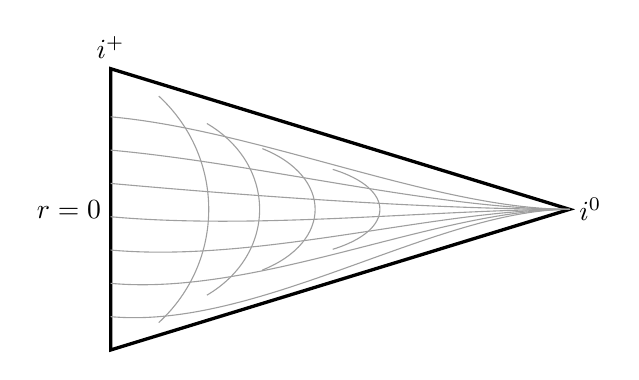
\begin{tikzpicture}[scale=0.94]
\coordinate (O) at (0,0);
\coordinate (P) at (0,3.8);
\coordinate (I) at (6.2,1.9);
\draw[very thick] (O)--(P)--(I)--cycle;
\foreach \y in {0.45,0.90,1.35,1.80,2.25,2.70,3.15} {
  \draw[gray!75] (0,\y) .. controls (2.0,\y-0.18) and (4.4,1.9) .. (I);
}
\draw[gray!75] (0.65,0.37) .. controls (1.55,1.20) and (1.55,2.60) .. (0.65,3.43);
\draw[gray!75] (1.30,0.74) .. controls (2.25,1.30) and (2.25,2.50) .. (1.30,3.06);
\draw[gray!75] (2.05,1.08) .. controls (3.00,1.46) and (3.00,2.34) .. (2.05,2.72);
\draw[gray!75] (3.00,1.36) .. controls (3.85,1.62) and (3.85,2.18) .. (3.00,2.44);
\node[left] at (0,1.9) {\(r=0\)};
\node[above] at (P) {\(i^+\)};
\node[right] at (I) {\(i^0\)};
\end{tikzpicture}
\caption{上部楔形の簡略版。曲線は定性的な定\(r\)および定\(t\)の族であり、正確な座標格子ではない。}
\label{fig:l05-flat-wedge}
\end{figure}

\(r\)を固定した世界線は、コンパクト化前は垂直であり、未来の時間的無限遠の近くで湾曲して蓄積する。定\(t\)のスライスも同様に空間的無限遠に向かって密集する。この密集は座標効果であり、物質の物理的な圧縮ではない。

\(45^\circ\)の規則は動径方向の光に直接適用される。角運動量をもつ光線は原点を外れ、ゼロでない最近接距離に達し、外向きに戻ることがある。原点から遠くでは、その射影された運動はほとんど動径的に見える。最近接の近くでのみ、還元された\((t,r)\)軌道が目に見えて曲がる。これで最初の作業部分は完了する。

\section{第二の作業部分：永遠のシュヴァルツシルト}

最大拡張シュヴァルツシルト解は、二つの外部ダイヤモンド、未来のブラックホール領域、および過去のホワイトホール領域をもつ。その上下の波状の境界は、未来および過去の特異点である。崩壊によって作られたブラックホールでは、この構造の大部分はまもなく捨てられるが、通常の右側の外部はまさに我々が必要とする部分である。

\begin{figure}[htbp]
\centering
\includegraphics[width=0.72\textwidth]{lecture_05_figure_03.png}
\caption{永遠のシュヴァルツシルト図。右側に通常の外部とその概略的な座標格子を示す。}
\lectureframe{00:16:55.975}
\end{figure}

\begin{figure}[htbp]
\centering
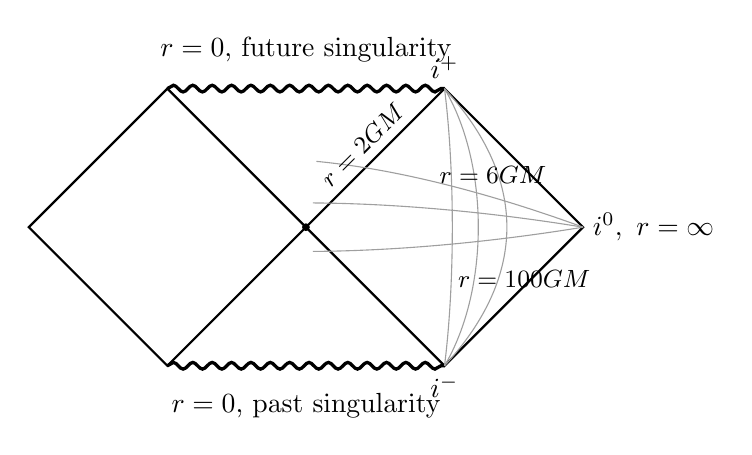
\begin{tikzpicture}[scale=0.88]
\coordinate (C) at (0,0);
\coordinate (TL) at (-2.0,2.0);
\coordinate (L) at (-4.0,0);
\coordinate (BL) at (-2.0,-2.0);
\coordinate (TR) at (2.0,2.0);
\coordinate (R) at (4.0,0);
\coordinate (BR) at (2.0,-2.0);
\draw[thick] (C)--(TL)--(L)--(BL)--(C);
\draw[thick] (C)--(TR)--(R)--(BR)--(C);
\draw[very thick,decorate,decoration={snake,amplitude=1.2pt,segment length=7pt}] (TL)--(TR);
\draw[very thick,decorate,decoration={snake,amplitude=1.2pt,segment length=7pt}] (BL)--(BR);
\draw[gray!75] (TR) .. controls (2.15,0.8) and (2.15,-0.8) .. (BR);
\draw[gray!75] (TR) .. controls (2.65,0.9) and (2.65,-0.9) .. (BR);
\draw[gray!75] (TR) .. controls (3.20,0.7) and (3.20,-0.7) .. (BR);
\draw[gray!75] (0.15,0.95) .. controls (1.5,0.82) and (2.9,0.40) .. (R);
\draw[gray!75] (0.10,0.35) .. controls (1.5,0.34) and (2.9,0.18) .. (R);
\draw[gray!75] (0.10,-0.35) .. controls (1.5,-0.34) and (2.9,-0.18) .. (R);
\fill (C) circle (1.6pt);
\node[above] at (TR) {\(i^+\)};
\node[below] at (BR) {\(i^-\)};
\node[right] at (R) {\(i^0,\ r=\infty\)};
\node[above] at (0,2.25) {\(r=0\), future singularity};
\node[below] at (0,-2.25) {\(r=0\), past singularity};
\node[rotate=45,above,font=\small] at (1.0,1.0) {\(r=2GM\)};
\node[font=\small] at (2.70,0.75) {\(r=6GM\)};
\node[font=\small] at (3.15,-0.75) {\(r=100GM\)};
\end{tikzpicture}
\caption{右側の外部は、大きな半径では平坦な楔形に似ている。その内側のヌル辺は\(c=1\)のとき\(r=2GM\)である。他のラベル付けされた半径は概略的な例である。}
\label{fig:l05-eternal-schwarzschild}
\end{figure}

ブラックホールから遠くでは、外部はますますコンパクト化された平坦空間のように見える。\(r=6GM\)や\(r=100GM\)のような線は、通常の定半径世界線の振る舞いに近づく。外部の内側の境界は
\begin{equation}
r=2GM
\end{equation}
であり、単位は\(c=1\)である。

中心の近くでは、平坦空間との比較は成り立たない。ミンコフスキー空間の動径光線は\(r=0\)に達し、反対側の物理的な側から再び現れる。シュヴァルツシルト内部の未来向き光線は跳ね返らない。それは\(r=0\)の空間的特異点で終わる。この因果的な違いこそ、崩壊の構成が保たなければならないものである。

\section{部分をつなぎ合わせることを可能にする定理}

欠けている要素はまずニュートン重力に現れる。球対称な質量分布に対して、ガウスの法則は
\begin{equation}
\oint\mathbf g\cdot d\mathbf A=-4\pi G M_{\mathrm{enc}},
\end{equation}
を与え、したがって
\begin{equation}
\mathbf g(r)=-\frac{G M_{\mathrm{enc}}(r)}{r^2}\,\hat{\mathbf r}.
\label{eq:l05-shell-theorem}
\end{equation}
となる。半径\(r\)の球の外側の物質は、そこに正味の場を寄与しない。全質量\(M\)の中空の殻に対しては、
\begin{equation}
\mathbf g=
\begin{cases}
0, & r<R_{\mathrm{shell}},\\[3pt]
-\dfrac{GM}{r^2}\hat{\mathbf r}, & r>R_{\mathrm{shell}}.
\end{cases}
\end{equation}

ビルクホフの定理はその相対論的な置き換えである。すべての球対称真空領域は、定数質量パラメータをもつ局所的なシュヴァルツシルト領域である。球殻の空の内部は質量パラメータがゼロで局所的にミンコフスキーであり、外部は質量パラメータ\(M\)をもちシュヴァルツシルトである：
\begin{equation}
\begin{aligned}
M_{\mathrm{enc}}&=0 && \text{inside the shell},\\
M_{\mathrm{enc}}&=M && \text{outside the shell}.
\end{aligned}
\label{eq:l05-birkhoff}
\end{equation}
この主張は殻が動いている間も有用であり続ける。なぜなら、両側の真空領域は球対称のままだからである。

\editorialnote{内部が平坦であることは局所的な主張である。静的な殻は、内部の曲率が消えていても、内部時間座標の規格化を変えうる。動く殻またはヌル殻に対しては、二つの真空計量を殻を挟んで接合しなければならない。理想化された構成は薄殻接合であり、内向きヴァイディヤ幾何と密接に関係している。これらの但し書きはいずれも、ここで用いられる因果的な切り貼り議論を変えない。}

実験室のイメージとしては、大きな慣性閉じ込め施設のように、同期したレーザーで密に覆われた球を想像し、それらをすべて一度に内向きに発射する。理想化では装置はなく、完全に球形の光の殻だけがある。殻はエネルギー\(E\)を運ぶので、外部の質量パラメータは
\begin{equation}
M=\frac{E}{c^2},
\end{equation}
であり、自然単位では単に\(E=M\)である。殻は光速で動くので、還元図上では内向きのヌル線である。その線上の各点は一つの光子の軌道ではなく、球面波面全体を表す。

\section{崩壊時空を縫い合わせる}

平坦な時空から始め、内向きのヌル殻を描く。殻の内側の領域は正しい。ビルクホフの定理によりそれは平坦である。外側の領域は正しくない。なぜなら、外部はそのシュヴァルツシルト幾何を通じて、すでに殻の全質量を知っていなければならないからである。

次に、同じ殻を永遠シュヴァルツシルト図に描こう。そこでは、殻の外側の領域は正しい。白色穴、第二の外部、そしてブラックホール内部の不適切な部分は、通常の空っぽの空間で始まる崩壊にとっては誤りであるから、それらを消去する。

\begin{figure}[htbp]
\centering
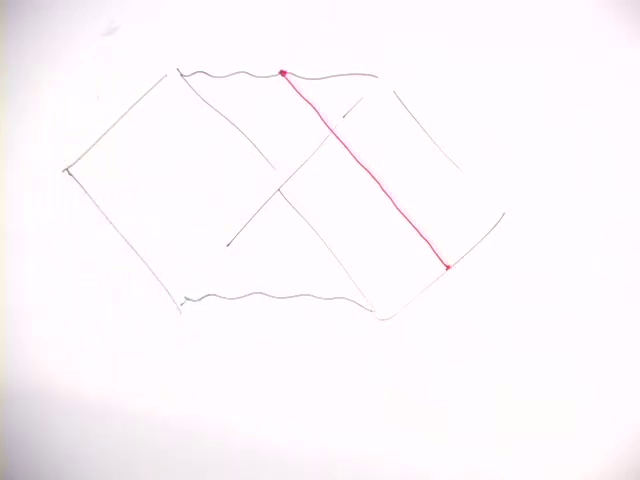
\includegraphics[width=0.72\textwidth]{lecture_05_figure_05.png}
\caption{赤で示されたヌル殻が、正しい外部部分を切り出しつつシュヴァルツシルト図全体に描かれている。}
\lectureframe{00:32:00.000}
\end{figure}

殻は平坦な部分において\(r=0\)に到達する。シュヴァルツシルト部分では、未来の特異点の始まりに到達する。これらは同じ端点である。平坦な内部を殻に沿ってシュヴァルツシルト外部に貼り合わせると、ブラックホール形成の最も単純な時空が得られる。

\begin{classroomqa}
\audiencequestion{左上の接合点において、平坦空間の端点は本当にシュヴァルツシルト側の点と同じなのですか。\lecturetimestamp{00:34:50}}
\lecturerresponse{はい。平坦空間の殻は\(r=0\)に収縮し、シュヴァルツシルト特異点もまた\(r=0\)にある。同定される二つの点は同じ幾何学的意味を持つ。すなわち、二次元球面が大きさゼロに収縮しているのである。}
\end{classroomqa}

\begin{figure}[htbp]
\centering
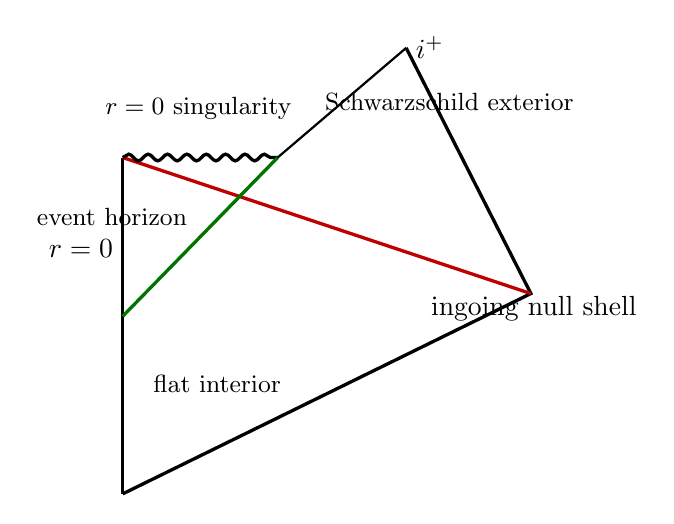
\begin{tikzpicture}[scale=0.96]
\coordinate (A) at (0,-2.8);
\coordinate (B) at (0,1.65);
\coordinate (C) at (2.05,1.65);
\coordinate (D) at (5.4,-0.15);
\coordinate (E) at (3.75,3.10);
\coordinate (H0) at (0,-0.45);
\draw[very thick] (A)--(B);
\draw[very thick] (A)--(D)--(E);
\draw[very thick,red!75!black] (D)--(B);
\draw[very thick,decorate,decoration={snake,amplitude=1.2pt,segment length=7pt}] (B)--(C);
\draw[very thick,green!45!black] (H0)--(C);
\draw[thick] (C)--(E);
\node[left] at (0,0.45) {\(r=0\)};
\node[below right] at (3.95,-0.05) {ingoing null shell};
\node[font=\small] at (1.25,-1.35) {flat interior};
\node[font=\small,anchor=west] at (2.55,2.38) {Schwarzschild exterior};
\node[above,font=\small] at (1.0,2.02) {\(r=0\) singularity};
\node[above left,font=\small] at (0.98,0.62) {event horizon};
\node[right] at (E) {\(i^+\)};
\end{tikzpicture}
\caption{崩壊の幾何。赤い殻は平坦な内部とシュヴァルツシルト外部を接合する。緑の事象の地平面は平坦領域においてより早く始まり、ブラックホール領域の未来境界で終わる。}
\label{fig:l05-collapse}
\end{figure}

この構成は、永遠解が残した問いに答える。崩壊から作られたブラックホールには、過去の白色穴も第二の漸近宇宙もない。それでも未来の特異点は持つ。

\section{地平面は大域的な境界である}

古いラベル\(r=2GM\)は、定常シュヴァルツシルト幾何において地平面を同定したが、それは動的時空で必要とされる定義ではない。

\begin{definition}
未来事象の地平面とは、未来向きの因果的信号を未来ヌル無限遠へ送ることができる事象の集合の境界である。
\end{definition}

崩壊図上で、ちょうど脱出に失敗する外向きヌル光線をたどろう。そのすぐ外側の光線は無限遠に到達し、すぐ内側の光線は特異点で終わる。その分離線が真の地平面である。

\begin{figure}[htbp]
\centering
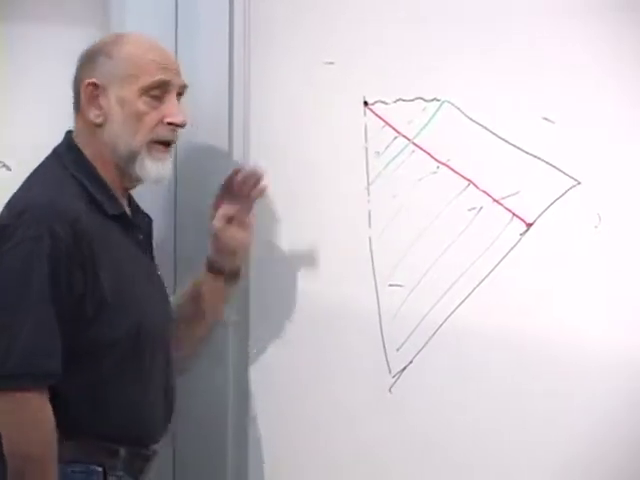
\includegraphics[width=0.72\textwidth]{lecture_05_figure_06.png}
\caption{完成した黒板の構成。入射する殻は赤、事象の地平面は緑であり、緑の線の一部は殻の下のまだ平坦な領域にある。}
\lectureframe{00:39:10.000}
\end{figure}

驚くべき特徴はもはや避けられない。地平面は、殻がまだ到着していない領域へと後方に延びている。そこの幾何は局所的に平坦であり、その線を横切る観測者は曲率のパルス、壁、閃光を検知しない。それにもかかわらず、その観測者はすでに無限遠に到達できない。なぜなら、未来の殻が可能な脱出経路をすべて閉ざすからである。事象の地平面はまさにこの大域的な意味で目的論的である。すなわち、それを見つけるには時空の未来全体の知識が必要である。\editorialnote{滑らかな事象の地平面をちょうど横切ったことを局所実験で決定することはできない。見かけの地平面やトラッピング地平面など他の概念はより局所的であり、崩壊の間、事象の地平面と一致する必要はない。}

排水口の類推は因果的考えを際立たせる。動かない湖の栓をした排水口の近くに漕ぎ手を想像しよう。栓が永遠に残るなら、漕ぎ手は去ることができる。誰かが必ず栓を抜くなら、まだ水が動いていなくても、後の流れが脱出を不可能にするかもしれない。凍結したナイアガラの滝も同じ点を示す。穏やかな水は安全への未来の経路を保証しない。

\begin{classroomqa}
\audiencequestion{光の球面殻がますます集中するから栓が抜かれるのですか。\lecturetimestamp{00:43:13}}
\lecturerresponse{その集中がブラックホールを創るが、排水口の話はより狭い目的で使われている。すなわち、局所的に劇的なことが何も起こる前に、すでに引き返せない点を越えていることがありうるのである。}
\end{classroomqa}

\subsection{成長する球面からなる地平面}

縮約された地平面の各点は\(S^2\)を表す。地平面の最初の点では、その球面は面積ゼロである。地平面に沿って上へ進むと、球面は成長し、その面積半径が
\begin{equation}
R_s=\frac{2GM}{c^2}.
\end{equation}
に達する。定常ブラックホールではその大きさにとどまり、さらにエネルギーが落下すれば再び成長する。

\editorialnote{理想化された球対称崩壊図では、地平面の生成子は\(r=0\)上の形成点、すなわち折り目で出会う。面積ゼロなのはこの極限の二次元球面であり、この記述は有限のシュヴァルツシルト地平面が突然一点に収縮すると読まれるべきではない。}

\subsection{遠方の観測者が再構成できること}

続く長い議論は、すでに大域的地平面の内側にいる観測者と、その観測者がそこに至るまでの歴史とを分ける。

\begin{classroomqa}
\audiencequestion{殻が到着する前に閉じ込められた人の状態はどうなっているのか。遠方の観測者から見て、その人は事象の地平面の外にいるのか。\lecturetimestamp{00:44:03}}
\lecturerresponse{いいえ。世界線が事象の地平面の背後に入ってしまえば、その未来は特異点に達し、そこから新たな信号が遠方の観測者に届くことはない。しかし、その人がそこで存在し始めたわけではない。それ以前の粒子、祖先、あるいは他の先行するエネルギーは、可視であった領域から入ってきたのである。}
\end{classroomqa}

したがって遠方の観測者は、先行する物質が地平面に近づくのを見ることができるが、その向こうから信号を受け取ることは決してない。到来する殻を通して見ることに矛盾はない。殻は光でできており、観測者は殻そのものも見て、ブラックホールが形成されたと推論できるのである。

\begin{classroomqa}
\audiencequestion{視線は崩壊する殻を通過するのか、そして外部の観測者は依然として穴が形成されたことを知ることができるのか。\lecturetimestamp{00:46:51}}
\lecturerresponse{はい。観測者は到来する殻を見ており、その光がまだ脱出できるうちに殻を横切る経路の光を受け取ることができる。奇妙に見えるのは、殻が中心に達する前から先行する物質が新たに定まった地平面に近づくことである。}
\end{classroomqa}

\begin{classroomqa}
\audiencequestion{これは、外部から見ると物質が地平面に圧縮されたように見えるという規則の続きなのか。\lecturetimestamp{00:47:49}}
\lecturerresponse{はい。外部記述では、物質は地平面に付随したままで、ますます赤方偏移し、やがてブラックホール蒸発という後の量子過程が話を変えるまで続く。}
\end{classroomqa}

この外部記述が次の主題を動機づける。情報が二次元の表面に貼り付けられているように見えるなら、ブラックホールのエントロピーがその表面の面積に比例することは、それほど驚くべきことではない。

\section{エントロピーと無限遠から見た温度}

大きな地平面の近くでは、小さな実験室で平坦地球近似を用いるのと同様に、球面を局所的な平面で置き換えてよい。そこで、以前の議論からの二つの事実が結び合わされる。
\begin{equation}
\begin{aligned}
S_{\mathrm{BH}}&\propto A_H,\\
\Delta A_H&\sim \ell_P^2
\quad\text{per added bit, schematically}.
\end{aligned}
\end{equation}
プランク面積あたり1ビットという記憶法は面積則を表しており、微視的な導出ではない。

シュヴァルツシルトブラックホールから遠く離れて測ったホーキング温度は
\begin{equation}
T_H=\frac{\hbar c^3}{8\pi GMk_B}.
\label{eq:l05-hawking}
\end{equation}
\(R_s=2GM/c^2\)を用いると、
\begin{equation}
T_H=\frac{\hbar c}{4\pi k_B R_s}.
\label{eq:l05-hawking-radius}
\end{equation}
したがって、より大きな穴はより冷たい。

\begin{classroomqa}
\audiencequestion{温度は位置に依存しうるのか。\lecturetimestamp{00:52:43}}
\lecturerresponse{日常的な会話では明らかに依存しうる。ニューヨークとスタンフォードが同じ温度である必要はない。より鋭い問いは、重力熱平衡にある系についてである。そこでは、赤方偏移した平衡温度が一定であっても、局所的な温度計の読みは高さによって変わりうる。}
\end{classroomqa}

温度は局所的な運動エネルギーを通して読み取られる。熱せられた地球の上の希薄な大気では、分子は上昇するにつれて運動エネルギーを失い、下降するにつれて得る。光子は上向きに赤方偏移し、下向きに青方偏移する。したがって、低い温度計と高い温度計は同じ局所的なエネルギー尺度を示す必要はない。

静的時空に対して、平衡関係は
\begin{equation}
T_{\mathrm{loc}}(r)\sqrt{-g_{tt}(r)}=T_\infty,
\label{eq:l05-tolman}
\end{equation}
すなわちトルマンの法則である。式~\eqref{eq:l05-hawking}のホーキング温度は\(T_\infty\)であり、無限遠で規格化された読みである。

\section{地平面近くの高温の静的雰囲気}

\(\rho\)を地平面から外向きの固有距離とする。大きなシュヴァルツシルト地平面の近くでは、式~\eqref{eq:l05-tolman}は
\begin{equation}
k_B T_{\mathrm{loc}}(\rho)
\simeq\frac{\hbar c}{2\pi\rho},
\label{eq:l05-local-temperature-si}
\end{equation}
となる。あるいは、単位\(c=\hbar=k_B=1\)では、
\begin{equation}
T_{\mathrm{loc}}(\rho)=\frac{1}{2\pi\rho}.
\label{eq:l05-local-temperature}
\end{equation}

\begin{figure}[htbp]
\centering
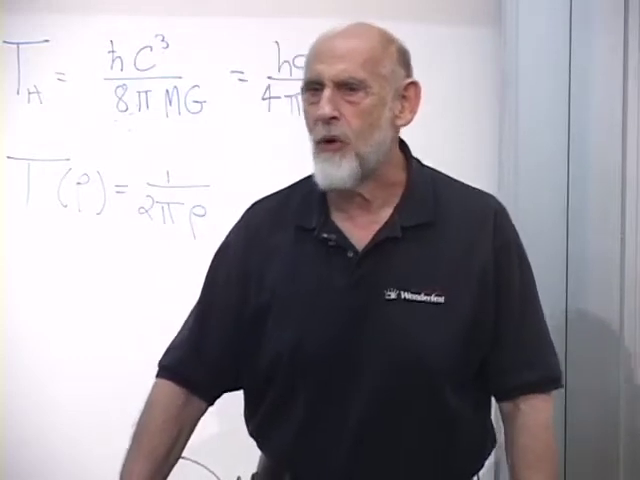
\includegraphics[width=0.72\textwidth]{lecture_05_figure_07.png}
\caption{漸近的なホーキング温度と、黒板に示された地平面近くの局所温度\(T(\rho)=1/(2\pi\rho)\)。}
\lectureframe{01:02:40.000}
\end{figure}

ケーブルで固定された\(\rho\)に保持された微小な温度計は、降ろされるにつれて上昇する温度を示す。その静的雰囲気中に保たれた原子は励起され、次に電離し、次に解離する。さらに大きな局所エネルギーでは、原子核やハドロンさえも無傷ではいられなくなる。人を足から先に降ろすと、記憶に残る診断が得られる。熱い足である。

\emph{保持された}という語が本質的である。この発散は、加速度によって静止させられた検出器に属する。それは外部時間に対して赤方偏移した熱的雰囲気を記述する。自由落下する検出器は異なる軌道をたどり、正則な量子状態にある十分大きな穴に対しては、地平面で発散する熱浴に出会う必要はない。\editorialnote{この区別は、静的観測者に見られるトルマン温度および加速度温度を、自由落下観測者の正則な局所経験から分かつ。講義はこの対比を、用語だけで解決するのではなく、意図的に操作的なパズルに変えている。}

電離の閾値がこの衝突を具体的にする。

\begin{classroomqa}
\audiencequestion{水素を電離するにはどれだけのエネルギーが必要か。\lecturetimestamp{01:06:53}}
\lecturerresponse{講義では\(13\)電子ボルトと答えられ、\(13.6\,\mathrm{eV}\)基底状態の電離エネルギーを正しく同定している。付随する数千ケルビンという見積もりは小さすぎるが、この議論には有限なしきい値が存在することだけが必要である。}
\end{classroomqa}

実際、
\begin{equation}
\frac{13.6\,\mathrm{eV}}{k_B}\simeq1.58\times10^5\,\mathrm{K}.
\end{equation}
したがって、静的温度が電離のスケールに達する小さな固有距離\(\rho_{\mathrm{ion}}\)が存在する。静的な外挿によれば、地平線の外側にあるその地点で原子はすでに電離しているはずである。これに対して自由落下する原子は、局所的な壁を予期せず、有限の固有時間で地平線を横切ることができる。外部の観測者は、これらの記述のどちらが正しいかを決める実験を行えるだろうか。

\section{ハイゼンベルクの顕微鏡}

この問いをブラックホールに適用する前に、光子顕微鏡を思い出そう。分解能\(\Delta x\)で粒子の位置を特定するには、探査波長は次を満たさなければならない。
\begin{equation}
\lambda\lesssim\Delta x.
\end{equation}
そのとき一つの光子は少なくとも次の運動量を運ぶ。
\begin{equation}
p_\gamma\gtrsim\frac{\hbar}{\Delta x}.
\label{eq:l05-microscope}
\end{equation}
その光子を散乱すると、同程度の反跳が生じる。まず位置を測定し、直ちに速度を調べると、二番目の測定は最初の測定によって変化した状態を見ることになる。実験は、排除しようとした条件を自ら作り出してしまう。

\begin{figure}[htbp]
\centering
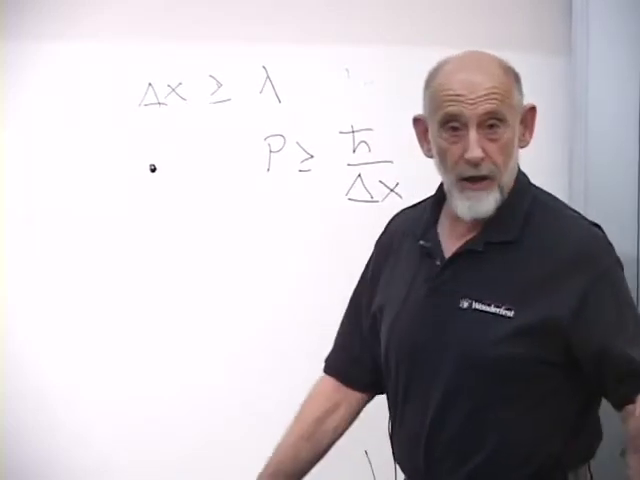
\includegraphics[width=0.70\textwidth]{lecture_05_figure_08.png}
\caption{顕微鏡は\(\Delta x\gtrsim\lambda\)および\(p_\gamma\gtrsim\hbar/\Delta x\)を見積もる。}
\lectureframe{01:11:50.000}
\end{figure}

これは単に古典光学の限界ではない。古典波はいくらでも弱くできるが、量子力学では検出が成功する事象に少なくとも一つの量子が必要である。したがって空間分解能を改善すれば、有限の運動量移行が不可避となる。

\section{地平線近傍の実験}

ここで、\(\rho_{\mathrm{ion}}\)から始まる層を原子が落下するとしよう。静的系に対して、それはほぼ\(c\)で内向きに運動しているので、地平線を横切るまでに利用できる間隔は次の程度である。
\begin{equation}
\Delta\tau\sim\frac{\rho_{\mathrm{ion}}}{c}.
\label{eq:l05-fall-time}
\end{equation}
横切った後は、いかなる結果も外部へ送り返すことはできない。測定は、この短い間隔の間に、無傷の原子と電離した原子を区別しなければならない。

層内で原子を分解するには次が必要である。
\begin{equation}
\lambda\lesssim\rho_{\mathrm{ion}}.
\end{equation}
したがって探査エネルギーは次で上限を付けられる。
\begin{equation}
E_\gamma=cp_\gamma
\gtrsim\frac{\hbar c}{\rho_{\mathrm{ion}}}.
\label{eq:l05-probe-energy}
\end{equation}
因子\(2\pi\)を除けば、これは式~\eqref{eq:l05-local-temperature-si}と同じスケールである。
\begin{equation}
E_\gamma\gtrsim2\pi k_B T_{\mathrm{loc}}(\rho_{\mathrm{ion}}).
\label{eq:l05-probe-temperature}
\end{equation}
事象を分解するのに十分なエネルギーを持つ光子は、原子を電離するのにも十分なエネルギーを持つ。

\begin{figure}[htbp]
\centering
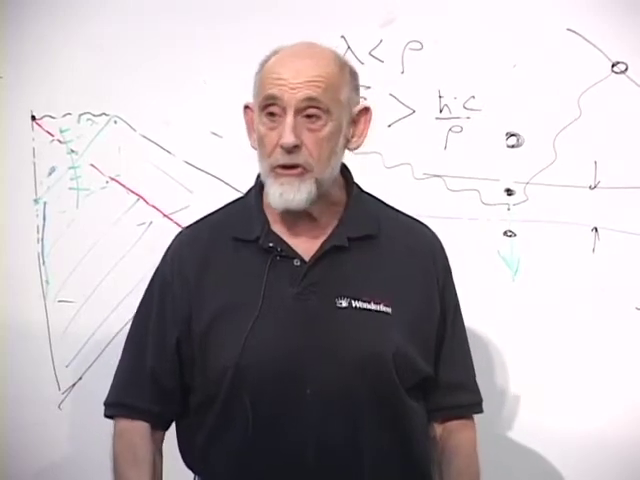
\includegraphics[width=0.72\textwidth]{lecture_05_figure_09.png}
\caption{黒板での地平線近傍の見積もり：\(\lambda<\rho\)は\(\hbar c/\rho\)程度の局所探査エネルギーを強制する。}
\lectureframe{01:18:30.000}
\end{figure}

\begin{classroomqa}
\audiencequestion{その高エネルギー光子は、自由落下系においてさえ原子を電離するだろうか。\lecturetimestamp{01:19:07}}
\lecturerresponse{はい。原子は実在の高エネルギー量子に衝突され、自身の局所系で反跳するか電離する。測定は乱されていない落下を明らかにするのではなく、それを乱された落下に置き換える。}
\end{classroomqa}

\begin{classroomqa}
\audiencequestion{原子が単に落下し、誰も実験を行わない場合はどうか。\lecturetimestamp{01:19:39}}
\lecturerresponse{その場合、この特定の擾乱は存在しない。外部の観測者が実際に高分解能の実験を行えば、原子は厄介なことになる。この議論は外部から検証できることに関するものであり、測定されない落下者が燃えることの証明ではない。}
\end{classroomqa}

\subsection{温度計や送信機の方がよりうまくできるだろうか。}

装置を移動しても情報の問題は解消しない。

\begin{classroomqa}
\audiencequestion{もっと遠くで測定し、勾配を推測し、あるいは自由落下する温度計に温度を記録させて後で回収することはできるだろうか。\lecturetimestamp{01:19:51}}
\lecturerresponse{地平線近傍の記録を知るには、何かが温度計と相互作用し、量子として情報を返さなければならない。温度計を引き返させるには激しい加速度が必要であり、遠隔で読み取るには放出か散乱が必要である。どちらの経路も、乱されていない履歴を検証しようとしていた物理系を変化させる。}
\end{classroomqa}

\begin{classroomqa}
\audiencequestion{小さな分解能に必要な高い探査エネルギーは、反射された観測を地平線近傍領域から遠ざけるのと同じ困難だろうか。\lecturetimestamp{01:21:51}}
\lecturerresponse{それらは同じ赤方偏移したスケールの両面である。光子は最終的に無限遠に達するときには低いエネルギーでありうる。なぜなら外へ登る間にエネルギーを失うからであるが、原子を分解する場所では高い局所振動数を持たなければならない。}
\end{classroomqa}

\editorialnote{地平線のすぐ外側で放出された光子は、単に脱出するためだけに大きなエネルギーを持つ必要はない。ここでの決定的な要件は、それが\(\rho\)程度の固有時間と距離のうちに事象を符号化することであり、重力赤方偏移がその大きな局所振動数をはるかに小さな漸近的振動数に関係づける。}

\begin{classroomqa}
\audiencequestion{物体が外部の光子に打たれるのではなく、自ら情報を放出することはできるのか。\lecturetimestamp{01:22:51}}
\lecturerresponse{できる。しかし、その局所的な放出にも、短い間隔の間に何が起きたかを同定するのに必要な帯域幅は依然として必要である。放出はまた、物体に反跳を与える。反射光を送信機で置き換えても、無コストの記録が得られるわけではない。}
\end{classroomqa}

\begin{classroomqa}
\audiencequestion{落下する原子には優先的な方向がある。その向きを持った運動エネルギーが温度と呼ばれているのか。\lecturetimestamp{01:23:10}}
\lecturerresponse{いいえ。野球ボールを投げても野球ボールは熱くならない。バルクの落下エネルギーと熱的揺らぎは別物である。この議論における温度は、原子の重心運動ではなく、周囲の静的放射大気に属するものである。}
\end{classroomqa}

\begin{classroomqa}
\audiencequestion{共に落下する実験室が磁場を用いて、原子が電離しているかどうかを調べることはできるか。\lecturetimestamp{01:23:50}}
\lecturerresponse{実験室は局所的な測定を行うことができる。困難は、地平線を横切る前にその結果を外部へ伝えることにある。その通信にもまた、相互作用と、必要な局所分解能を持つ外向きの量子が必要である。}
\end{classroomqa}

\begin{classroomqa}
\audiencequestion{温度計に組み込まれた送信機は、装置を破壊してしまうほど多くの局所エネルギーを必要とするのか。\lecturetimestamp{01:24:57}}
\lecturerresponse{それは同じ障害を工学的な形で表したものである。地平線に十分近づくと、関連する局所スケールで必要となる信号エネルギーは、測定しようとしている熱的スケールと同程度になる。}
\end{classroomqa}

\begin{classroomqa}
\audiencequestion{高温領域は、ゆっくり測定を行う時間がないほど薄いのか。\lecturetimestamp{01:25:15}}
\lecturerresponse{そのとおり。その固有の厚さは\(\rho\)の程度であり、横断時間は\(\rho/c\)の程度である。この制限は空間分解能としても時間帯域幅としても記述できるが、どちらの記述でも高い局所運動量またはエネルギーを要求する。}
\end{classroomqa}

対応する時間帯域幅の評価は
\begin{equation}
\Delta E\,\Delta\tau\gtrsim\hbar.
\end{equation}
である。ここではこれはフーリエ分解能または操作的な分解能の限界として読まれるべきであり、\(\Delta x\,\Delta p\geq\hbar/2\)と同一の地位を持つ演算子の不確定性関係としてではない。講義は時間とエネルギーの不確定性を発見法的に用いている。空間分解能から導かれた式~\eqref{eq:l05-probe-energy}が、この議論のより堅固な部分である。

\begin{classroomqa}
\audiencequestion{より低エネルギーで低分解能のプローブを多数の原子に用い、統計的に答えを回復することはできるか。\lecturetimestamp{01:26:26}}
\lecturerresponse{これはもっともな問いであり、教室では未解決のままにされている。各原子はただ一度の通過しか与えず、回復される信号は依然として、地平線近傍の短い事象を同定するのに十分な情報を運ばなければならない。講義は不確定性原理に訴えているが、完全な統計的ノーゴー証明を与えてはいない。}
\end{classroomqa}

\enlargethispage{2\baselineskip}
\section{何が確立され、何が確立されていないか}

この議論は、自由落下する人が発散する静的温度を感じなければならないと予測しているのではない。

\begin{classroomqa}
\audiencequestion{落下する人は温度を感じないと予測できると言っているのか。\lecturetimestamp{01:27:38}}
\lecturerresponse{いいえ。結論はもっと狭い。原子が高温の擾乱を経験しなかったことを確認するために設計された外部の実験は、同じスケールの擾乱を生み出す、ということである。この操作的解析が確立するのはそれだけである。}
\end{classroomqa}

したがって結論は、ファイアウォール定理でも、落下者が焼かれることの証明でも、何も起こらないことの証明でもない。それは外部からの検証に対する限界である。すなわち、\emph{擾乱されていない地平線近傍の事象を分解するには、それを擾乱するプローブが必要である}。
実験を行えば、その量子は、試験しようとしていた効果を生み出す。実験を行わなければ、この議論だけでは、実験的にアクセス可能な追加の事実を何も与えない。二重スリット実験との比較は意図的なものである。経路測定なしにどちらのスリットを通ったかを問うことと、相互作用なしに外部装置が何を証明するかを問うことは、どちらも、提案された証拠が得られないところに操作的な答えを結びつけようとする試みである。
